\chapter{Upload dan Pull Pada Image}

\begin{figure}
\section{Pembuka}
Panduan kali ini membahas upload dan pull docker images. Upload yang dilakukan yaitu menyimpan docker images yang sudah dibuat ke repositori Docker Hub.
Push merupakan perintah docker untuk mengupload docker image ke repositori akun docker hub. 
Pull yang dilakukan yaitu mengambil docker images yang sudah ada di docker registri ke penyimpanan lokal untuk digunakan. 
Pull merupakan perintah docker untuk mengambil docker images yang tersedia di docker registry. Dengan ini pengguna tidak perlu membuat Dockerfile untuk membuat docker image, cukup download saja yang sudah tersedia.

    \section{Upload Image ke Docker Hub}

    1. Buat akun pada Docker Hub/apabila sudah ada lakukan login ke Docker Hub, kemudian buat repositori baru dengan klik tombol CREATE REPOSITORY
        \begin{center}
            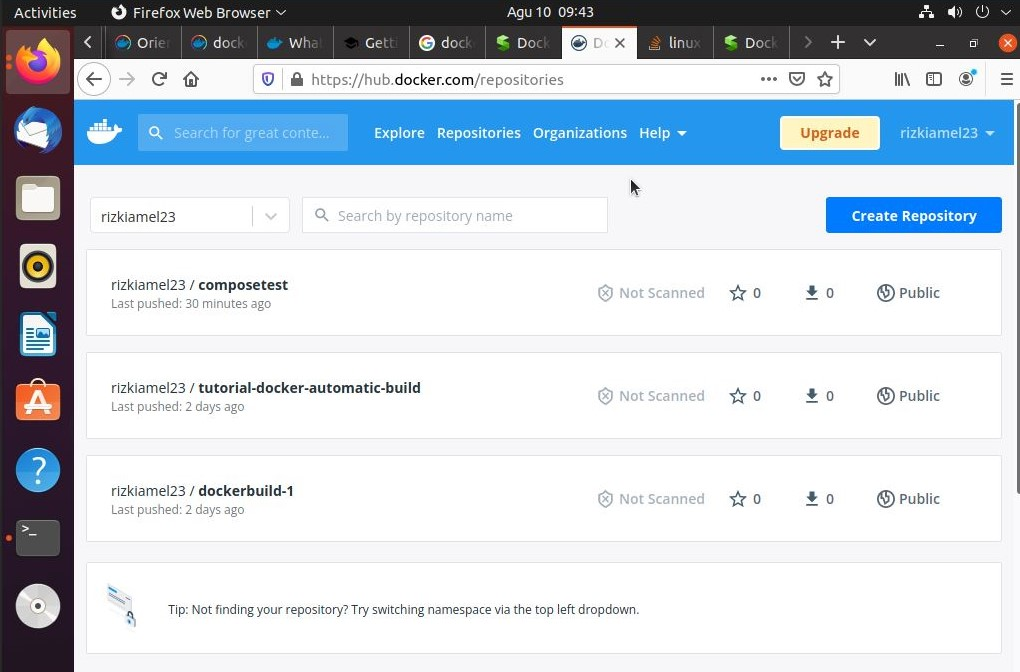
\includegraphics[width=\linewidth]{image/26.jpg}
            \caption{Buat repositori docker hub}
            \label{fig:my_figure}
        \end{center}

\end{figure}
\begin{figure}
    2. Beri nama repositori sesuai dengan nama docker images yang sudah dibuat, tambahkan deskripsi(opsional), atur akes public/private, lalu klik tombol CREATE
        \begin{center}
            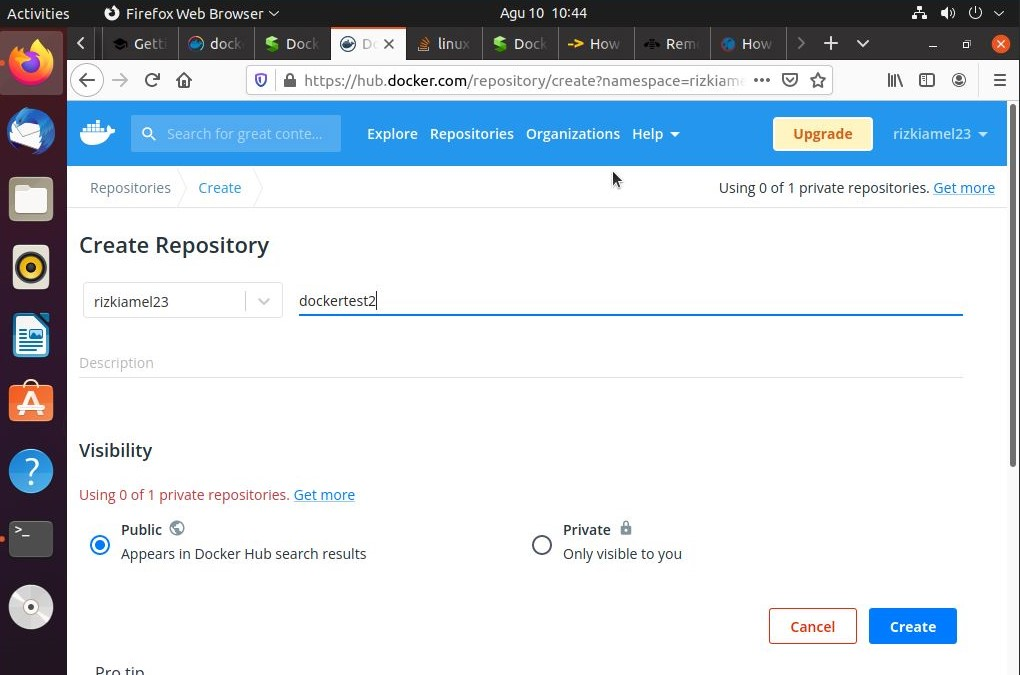
\includegraphics[width=\linewidth]{image/27.jpg}
            \caption{Pengaturan repositori}
            \label{fig:my_figure}
        \end{center}

    3. Jika berhasil maka tampilan terlihat seperti berikut 
        \begin{center}
            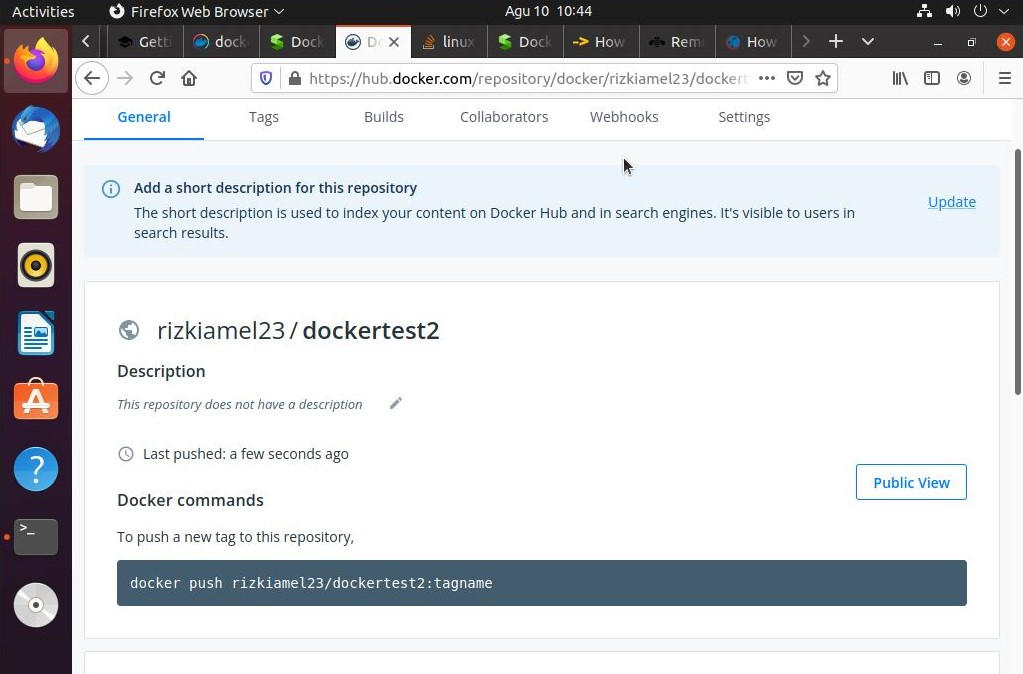
\includegraphics[width=\linewidth]{image/28.jpg}
            \caption{Berhasil membuat repositori}
            \label{fig:my_figure}
        \end{center}
\end{figure}
\begin{figure}
    4. Lakukan login dengan akun docker di command line

    COMMAND: \textcolor{Blue}{docker login}, masukan USERNAME dan PASSWORD, klik ENTER, jika berhasil akan menampilkan login succeded
        \begin{center}
            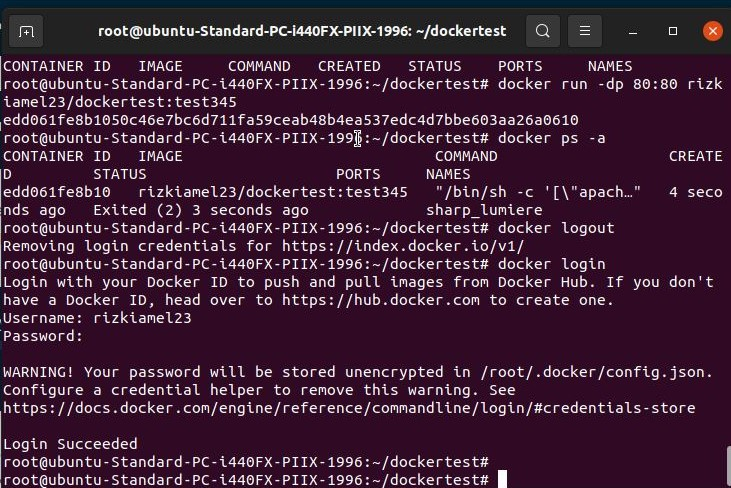
\includegraphics[width=\linewidth]{image/30.jpg}
            \caption{Login docker di command line}
            \label{fig:my_figure}
        \end{center}
    5. Lakukan upload docker image ke repositori docker hub yang sudah dibuat
    
    Lakukan upload image : \textcolor{Gray}{docker push <NAMA IMAGE:TAG>}
        
    COMMAND: \textcolor{Blue}{docker push rizkiamel23/dockertest2:test567}
        \begin{center}
            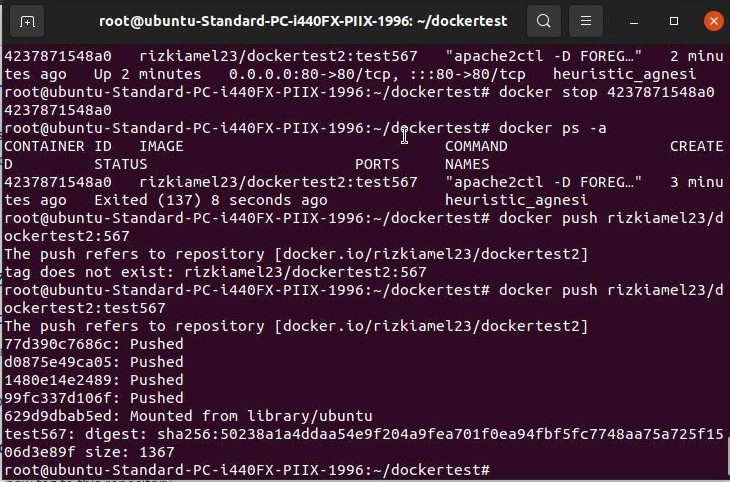
\includegraphics[width=\linewidth]{image/32.jpg}
            \caption{Upload docker images}
            \label{fig:my_figure}
        \end{center}
\end{figure}
    
\begin{figure}
    6. Buka docker hub pada browser, jika berhasil pada tab tag and scans akan menampilkan tag dari image yang sudah diupload tadi
        \begin{center}
            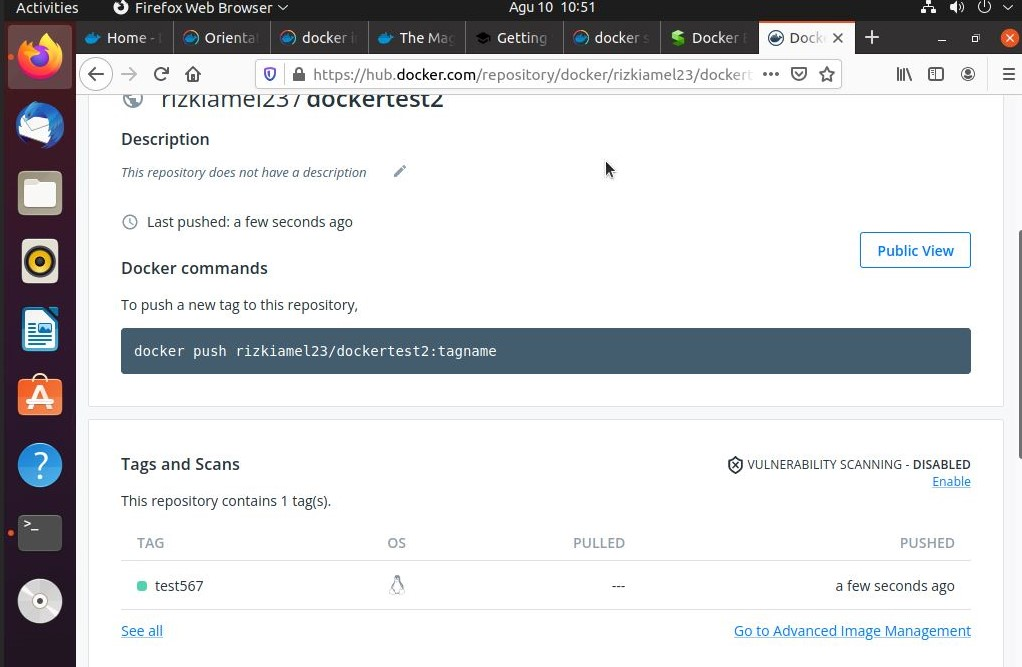
\includegraphics[width=\linewidth]{image/33.jpg}
            \caption{Tampilan berhasil upload}
            \label{fig:my_figure}
        \end{center}
\end{figure}

\begin{figure}
\section{Pull Image dari Docker Registry}

1. Pull image debian dari docker repositori

Pull image debian : \textcolor{Gray}{docker pull <IMAGE NAME:TAG>}

COMMAND: \textcolor{Blue}{docker pull debian:latest}

Cek docker images setelahnya 

COMMAND: \textcolor{Blue}{docker images}
    \begin{center}
        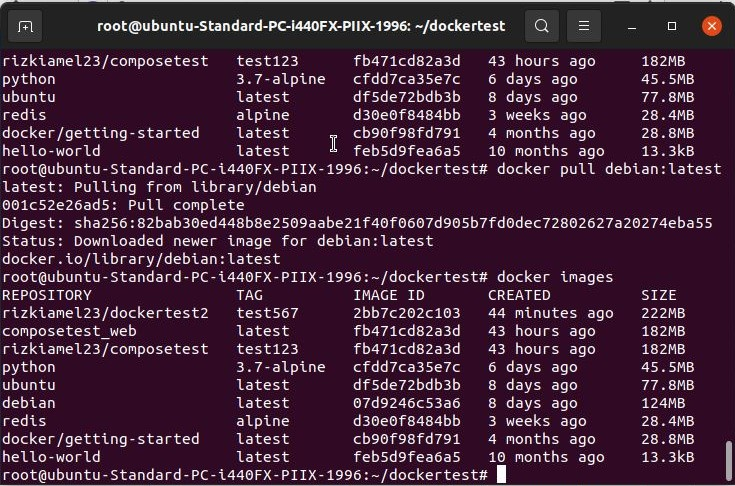
\includegraphics[width=\linewidth]{image/35.jpg}
        \caption{Pull docker images}
        \label{fig:my_figure}
    \end{center}

Setelah docker image di pull/diambil, pengguna dapat membangun kontainer seperti biasa dari 
docker image yang telah di pull dari registri.

\end{figure}



